\documentclass{article}
\pdfpagewidth=8.5in
\pdfpageheight=11in

\usepackage{POBRreport}
% Use the postscript times font!
\usepackage{times}
\usepackage{soul}
\usepackage{url}
\usepackage{xcolor}
\usepackage{polski}
\usepackage[polish]{babel}
\usepackage[utf8]{inputenc}
\usepackage[T1]{fontenc}
\usepackage[utf8]{luainputenc}
\usepackage[hidelinks]{hyperref}
\usepackage[utf8]{inputenc}
\usepackage{caption}
\usepackage{indentfirst}
\usepackage{graphicx}
\usepackage{amsmath}
\usepackage{siunitx}
\usepackage{booktabs}
\urlstyle{same}

\title{Przetwarzanie Cyfrowe Obrazów \\ Wykrywanie logo restauracji Burger King}

\author{
Jakub Sikora
\affiliations
nr albumu: 283418\\
\emails
jakub.sikora2.stud@pw.edu.pl
}

\newcommand{\bk}{
    Burger King
}
\newcommand{\todo}[1]{\textcolor{blue}{\textbf{TO DO:} #1}}

\begin{document}

\maketitle

\section{Treść zadania}
\label{sec:cel-projektu}
Celem projektu jest praktyczne zapoznanie się studentów z cyfrowymi metodami przetwarzania, analizy i rozpoznawania obrazów. 

Dla obrazów zawierających logo restauracji \bk należy dobrać, zaimplementować i przetestować odpowiednie procedury wstępnego przetworzenia, segmentacji, wyznaczania cech oraz identyfikacji obrazów cyfrowych. Powstały w wyniku projektu program powinien poprawnie rozpoznawać wybrane obiekty dla reprezentatywnego zestawu obrazów wejściowych. W trakcie projektu należy przetestować wybrane algorytmy i ocenić ich praktyczną przydatność. Wnioski powstałe w trakcie projektu muszą zostać przedstawione w formie pisemnego sprawozdania. Zaliczenie projektu dokonywane jest na podstawie pokazu działania zrealizowanego programu oraz sprawozdania. Sprawozdanie ma zawierać wyszczególnienie wybranych i zaimplementowanych algorytmów oraz wnioski powstałe w trakcie implementacji i testowania programu.

Jako dane wejściowe muszą być wykorzystane: zdjęcia w postaci papierowej - wykonane własnoręcznie lub wybrane np. z książek i czasopism, które należy zeskanować; lub zdjęcia w postaci cyfrowej - uzyskane za pomocą aparatu cyfrowego. Danych wejściowych nie mogą stanowić obrazy uzyskane bezpośrednio cyfrowo tzn. np. z programów typu MS Paint, Corel Draw itp. Ponadto w projekcie nie można wykorzystywać funkcji bibliotecznych do przetwarzania, analizy oraz rozpoznawania obrazów.


\section{Logo restauracji \bk}
\label{sec:logo-bk}
Przedstawione na rysunku \ref{fig:bklogo} logo restauracji \bk składa się z~czterech części:
\begin{itemize}
    \item czerwonego napisu \bk,
    \item żółtej bułki od burgera podzielonej na pół,
    \item niebieskiej paska okalającego napis,
    \item białego okrągłego tła.
\end{itemize}

\begin{figure}[tb]
    \centering
    
\includegraphics[width=0.4\columnwidth]{./figures/bklogo.pdf}
    \caption{Logo restauracji \bk~\cite{WikipediaEN:bklogo}}
    \label{fig:bklogo}
\end{figure}

Każda z~części ma swoją stałą, rozróżnialną barwę, co pozwala ją w~pełni rozróżnić od innych elementów. Poszczególne elementy praktycznie nienachodzą na siebie, nie licząc kawałka czerwonego napisu zachodzącego na fragment niebieskiej obwódki. Logo jest wpisane w~okrąg, dzięki czemu dobrze skaluje się w~przestrzeni.

Typowo, logo \bk można znaleźć na elewacjach budynków tej restauracji, na znakach przydrożnych oraz wewnątrz samej restauracji. Co więcej, logo może być przedstawione z~wewnętrznym podświetleniem lub bez niego. Powoduje to bardzo zmienne warunki oświetleniowe znaku, co mimo prostego zestawu barw, czyni z~niego ciekawy obiekt do automatycznego wykrywania.


\section{Zarys algorytmu przetwarzania}
\label{sec:algorytm}
\todo{Opisać zgrubnie jak przetwarzany będzie obraz, w celu wykrycia logo \bk. Przygotować schemat blokowy rozwiązania. Napisać że to implementacja w C++}

Ogólnie w~algorytmie można wydzielić pięć odrębnych faz przetwarzania. Poszczególne fazy zostały zaprezentowane za pomocą schematu blokowego na rysunku~\ref{fig:algorithm-overview}.

\begin{figure}
    \centering
    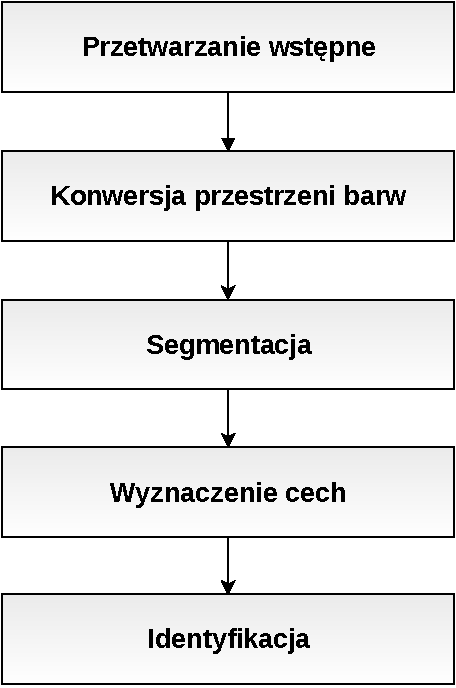
\includegraphics[width=0.6\columnwidth]{figures/algorithmOverview.pdf}
    \caption{Ogólny schemat blokowy algorytmu wykrywania logo \bk}
    \label{fig:algorithm-overview}
\end{figure}

\section{Przetwarzanie wstępne}
\label{sec:preprocessing}
\todo{Opisać algorytmy przetwarzania wstępnego. Dać źródła i opisać implementację.}

\subsection{Skalowanie obrazu}
\todo{Opisać algorytm skalowania obrazu - interpolacji dwuliniowej. Znaleźć źródła. Opisać inne algorytmy skalowania obrazu. }

\subsection{Filtracja zakłóceń}
\todo{Opisać algorytm filtracji zakłóceń - filtracja medianowa. Znaleźć źródła.}

\section{Konwersja przestrzeni barw}
\label{sec:przestrzenie}
Po przetwarzaniu wstępnym obrazu, kolejnym krokiem algorytmu wykrywania logo \bk była konwersja przestrzeni barw z~RGB do przestrzeni~HSV.

\subsection{Przestrzeń RGB}
Najbardziej znanym modelem przestrzeni barw jest model opisywany współrzędnymi RGB. Nazwa współrzędnych pochodzi od pierwszych liter nazw barw podstawowych: \textbf{R} - czerwona, \textbf{G} - zielona oraz \textbf{B} - niebieska. Model ten bazuje na właściwościach ludzkiego oka. Wrażenie widzenia dowolnej barwy można uzyskać poprzez zmieszanie trzech wiązek światła \cite{jankowski1990elementy}.

Model RGB jest domyślnie wykorzystywany w~informatyce do przechowywania plików graficznych. Wykorzystywana w~rozwiązaniu biblioteka OpenCV, również bazuje na tym modelu, odwracając kolejność kolorów. Zamiast jako pierwszą przechowywać informację o kolorze czerwonym, pierwsza przechowywana informacja mówi o~kolorze niebieskim, tak jak zostało to przedstawione na rysunku~\ref{fig:bgr}. Tak odwróconą przestrzeń nazywa się przestrzenią BGR~\cite{opencv}.

\begin{figure}[h]
    \centering
    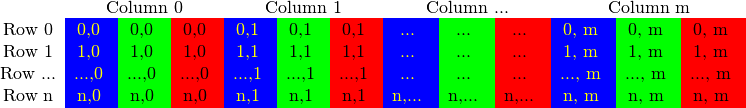
\includegraphics[width=\columnwidth]{./figures/opencv-matrix-bgr.png}
    \caption{Sposób reprezentacji obrazu w~przestrzeni BGR, wykorzystywanej w~OpenCV~\cite{opencv}}
    \label{fig:bgr}
\end{figure}

\subsection{Przestrzeń HSV}
Model HSV czerpie swoją nazwę od pierwszych liter angielskich nazw składowych: \textbf{H} - hue (barwa), \textbf{S} - saturation (nasycenie), \textbf{V} - value (wartość). Model ten znacznie różni się od poprzednio omawianego modelu. W~RGB, wszystkie trzy zmienne niosą jednocześnie informację na temat chrominancji (kolorze) i~luminancji (jasności) punktu. W~modelu HSV, tylko jedna składowa \textbf{V} niesie informację o~jasności piksela a~pozostałe dwie zmienne \textbf{H}~i~\textbf{S}~przechowują informację o~chrominancji piksela. Taki sposób reprezentacji znacznie ułatwia wykrywanie na zdjęciu obiektów o~danej barwie lecz o~różnym oświetleniu. Typowo, przestrzeń HSV przedstawia się za pomocą stożka, zaprezentowanego na rysunku~\ref{fig:hsv}.

\begin{figure}[h]
    \centering
    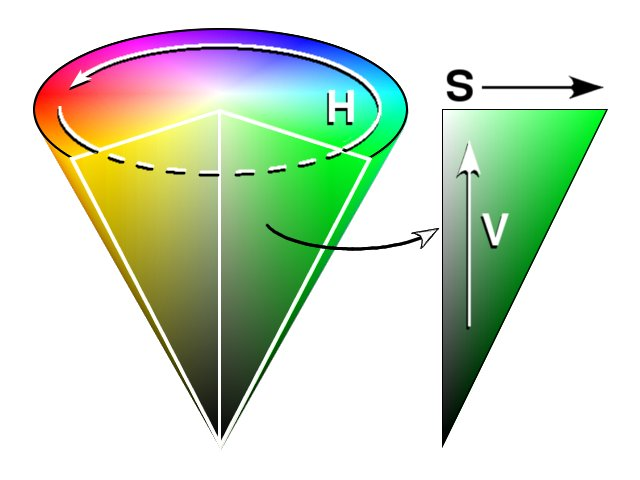
\includegraphics[width=0.6\columnwidth]{./figures/HSV_cone.jpg}
    \caption{Stożek przestrzeni barw HSV~\cite{WikipediaPL:hsvCone}}
    \label{fig:hsv}
\end{figure}   

Podobnym modelem do HSV jest model HSL (\textit{Hue, Saturation, Lightness}). Oba modele jednakowo definiują zmienną barwową H, natomiast różnią się w~definicji pozostałych zmiennych. Największe różnice zachodzą w~definicji jasności/wartości koloru. W~modelu HSV, wartość $0\%$ reprezentuje kolor czarny, natomiast wartość $100\%$ kolor w pełni nasycony. W~modelu HSL, w~pełni nasycone kolory mają wartość jasności $50\%$, natomiast kolory czarny i~biały mają odpowiednio $0\%$ oraz $100\%$. Mimo iż model HSL bardziej intuicyjnie przedstawia jasność koloru, uznałem że bardziej odpowiedni do automatycznego przetwarzania będzie model HSV.

\subsection{Implementacja konwersji}
Konwersja piksela w~modelu RGB $(R, G, B)$ do modelu HSV $(H,S,V)$ jest operacją punktową i~nie wymaga informacji na temat wartości innych pikseli. W~programie, konwersję przeprowadza obiekt klasy \texttt{POBR::BGR2HSVConverter}. 

Pierwszym krokiem algorytmu konwersji jest obliczenie jasności $V$, zgodnie ze wzorem \ref{eqn:value}.
\smallskip
\begin{equation}
    \label{eqn:value}
    V = \max{(R, G, B)}
\end{equation}

Kolejnym krokiem algorytmu, jest obliczenie nasycenia koloru $S$, korzystając ze wzoru~\ref{eqn:saturation}.

\begin{equation}
    \label{eqn:saturation}
    S = \left\{ 
        \begin{array}{ll}
            0, & V = 0 \\
            \min{(R, G, B)}, & V \ne 0
        \end{array} 
        \right.
\end{equation}

Ostatnim krokiem algorytmu jest obliczenie barwy $H$~zgodnie z~wzorem~\ref{eqn:hue}.

\begin{equation}
    \label{eqn:hue}
    H = \left\{ 
        \begin{array}{ll}
            \frac{(G - B) * 60\si{\degree}}{V - \min{(R, G, B)}} + 60\si{\degree}, & V = R \\
            \frac{(B - R) * 60\si{\degree}}{V - \min{(R, G, B)}} + 120\si{\degree}, & V = G \\
            \frac{(R - G) * 60\si{\degree}}{V - \min{(R, G, B)}} + 240\si{\degree}, & V = B
        \end{array} 
        \right.
\end{equation}
\smallskip

Wartości zmiennych $V$~i~$S$ mieszczą się w~przedziale $[0; 255]$ natomiast wartości zmiennej $H$ są ograniczone przez przedział $[0; 360]$. Obrazy przechowywane są tablicy o~ośmiobitowym rozmiarze podstawowym \texttt{uchar}. Zmienna $H$ nie mieści się w~komórce o~tym rozmiarze, dlatego też zdecydowałem się na przechowywanie w~tablicy wartości $\frac{H}{2}$. Podział ten jest solidnym kompromisem pomiędzy dokładnością reprezentacji a~rozmiarem obrazu w~pamięci komputera. Jest on również domyślnie wykorzystywany w~reprezentacji obrazów w~modelu~HSV w~bibliotece OpenCV~\cite{opencv}.

\section{Segmentacja}
\label{sec:segmentacja}
\todo{Opisać na schemacie blokowym lub sekwencji (jeśli będzie wielowątkowo) jak działa rozwiązanie progowania kolorów.}
\todo{Opisać algorytm segmentacji obrazu - rozrost obszarów najpewniej}


\section{Wyznaczenie cech}
\label{sec:wyznaczanie-cech}
\todo{Opisać algorytm wyznaczania cech segmentów oraz jakie cechy zostały wyznaczone. Podeprzeć się tym co wyznacza matlab.}

\section{Identyfikacja}
\label{sec:identyfikacja-cech}
\todo{Opisać algorytm identyfikacji segmentów z wyznaczonymi cechami.}


\section{Podsumowanie}
\label{sec:podsumowanie}
\todo{Króciutkie podsumowanie że projekt był fajny i takie tam}

\bibliographystyle{abbrv}
\bibliography{bibliography}

\end{document}